\chapter{Building Simulation Programs}
\label{cha:building-simulation-programs}




\section{Overview}

As it was already mentioned, an {\opp} model physically consists of
the following parts:
\begin{itemize}
  \item{NED language\index{ned!files} topology description(s). These
      are files with the \ttt{.ned} suffix.}
  \item{Message definitions\index{message definitions}, in files
      with \ttt{.msg} suffix.}
  \item{Simple modules implementations and other C++ code, in \ttt{.cc}
        files (or \ttt{.cpp}, on Windows)}
\end{itemize}


To build an executable simulation program,
you first need to translate the NED files\index{ned!files}
and the message files into C++, using the NED compiler\index{ned!compiler}
(\ttt{nedc}) and the message compiler (\ttt{opp\_msgc}).
After this step, the process is the same as building any C/C++
program from source: all C++ sources need to be compiled into object files
(\ttt{.o} files on Unix/Linux, and \ttt{.obj} on Windows),
and all object files need to be linked with the necessary libraries to get
an executable.

%%  \footnote{Future versions of {\opp} may support runtime loading
%%  of NED files, so that you do not have to recompile.}

File names for libraries differ for Unix/Linux and for Windows,
and also different for static and shared libraries.
Let us suppose you have a library called Tkenv.
On a Unix/Linux system, the file name for the static library
would be something like \ttt{libtkenv.a} (or \ttt{libtkenv.a.}\textit{<version>}),
and the shared library would be called \ttt{libtkenv.so}
(or \ttt{libtkenv.so.}\textit{<version>}).
The Windows version of the static library would be \ttt{tkenv.lib},
and the DLL (which is the Windows equivalent of shared libraries)
would be a file named \ttt{tkenv.dll}.

You'll need to link with the following libraries:

\begin{itemize}
  \item{The simulation kernel and class library\index{simulation!kernel},
    called \textit{sim\_std} (file \ttt{libsim\_std.a}, \ttt{sim\_std.lib}, etc).}
  \item{User interfaces. The common part of all user interfaces is
    the \textit{envir} library (file \texttt{libenvir.a}, etc),
    and the specific user interfaces are \textit{tkenv} and \textit{cmdenv}
    (\ttt{libtkenv.a}, \ttt{libcmdenv.a}, etc). You have to link
    with \textit{envir}, plus either \textit{tkenv} or \textit{cmdenv}.}
\end{itemize}

Luckily, you do not have to worry about the above details, because
automatic tools like \ttt{opp\_makemake} will take care of the hard
part for you.

The following figure gives an overview of the process of building
and running simulation programs.

\begin{figure}[htbp]
  \begin{center}
    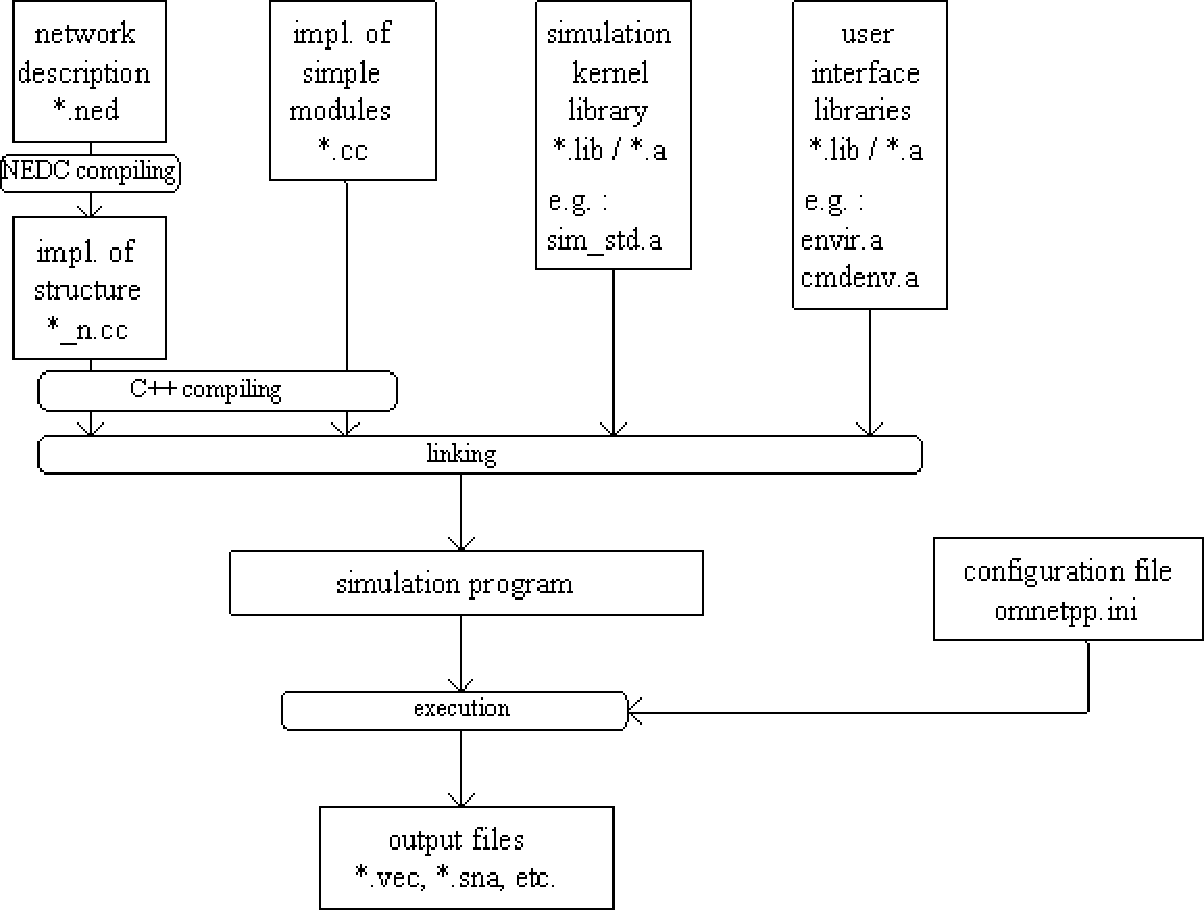
\includegraphics[width=5.992in, height=4.519in]{figures/usmanFig17}
    \caption{Building and running simulation}
  \end{center}
\end{figure}


This section discusses how to use the simulation system on the
following platforms:
\begin{itemize}
  \item{Unix with gcc (also Windows with Cygwin or MinGW)}
  \item{MSVC 6.0 on Windows}
\end{itemize}




\section{Using Unix and gcc}

This section applies to using {\opp} on Linux, Solaris, FreeBSD and
other Unix derivatives, and also more or less to Cygwin and MinGW
on Windows.

Here in the manual we can give you a rough overview only.
The \ttt{doc/} directory of your {\opp} installation contains
\ttt{Readme.}\textit{<platform>} files that provide
up-to-date, more detailed and more precise instructions.


\subsection{Installation}

The installation process depends on what distribution you take
(source, precompiled RPM, etc.) and it may change from release
to release, so it is better to refer to the readme files.
If you compile from source, you can expect the usual GNU
procedure: \ttt{./configure} followed by \ttt{make}.


\subsection{Building simulation models}

The \fprog{opp\_makemake} script can automatically generate the
\texttt{Makefile} for your simulation program, based on the source files
in the current directory. (It can also handle large models
which are spread across several directories; this is covered later in
this section.)

\fprog{opp\_makemake} has several options, with the \ttt{-h}
option it displays a summary.

\begin{verbatim}
% opp_makemake -h
\end{verbatim}

Once you have the source files (\ttt{*.ned}, \ttt{*.msg}, \ttt{*.cc},
\ttt{*.h}) in a directory, \ttt{cd} there then type:

\begin{verbatim}
% opp_makemake
\end{verbatim}

This will create a file named \texttt{Makefile}\index{Makefile}. Thus if you
simply type \fprog{make}, your simulation program should build. The name of
the executable will be the same as the name of the directory
containing the files.


The freshly generated \texttt{Makefile} doesn't contain
dependencies\index{Makefile!dependencies}, it is advisable to add them
by typing \fprog[make]{make depend}. The warnings during the
dependency generation process can be safely ignored.

In addition to the simulation executable, the \texttt{Makefile}
contains other targets, too. Here is a list of important ones:

\begin{longtable}{|l|p{8cm}|}
\hline
\tabheadcol
\tbf{Target} & \tbf{Action}\\\hline
 & The default target is to build the simulation executable\\\hline
depend & Adds (or refreshes) dependencies in the \texttt{Makefile}\\\hline
clean &  Deletes all files that were produced by the make process\\\hline
makefiles & Regenerates the \texttt{Makefile} using \fprog[make]{opp\_makemake} (this is useful if e.g.  after upgrading {\opp}, if \fprog{opp\_makemake} has changed)\\\hline
makefile-ins & Similar to \fprog[make]{make makefiles}, but it regenerates the \texttt{Makefile.in} instead\\\hline
\end{longtable}

If you already had a \texttt{Makefile} in that directory, \fprog{opp\_makemake}
will refuse to overwrite it. You can force overwriting the old \texttt{Makefile}
with the -f option:

\begin{verbatim}
% opp_makemake -f
\end{verbatim}

If you have problems, check the path definitions (locations of include
files and libraries etc.) in the configure script\index{configure script}
and correct them if necessary. Then re-run configure for the changes
to take effect.

You can specify the user interface (Cmdenv/Tkenv) with the -u option
(with no -u, Tkenv is the default):

\begin{verbatim}
% opp_makemake -u Tkenv
\end{verbatim}

Or:

\begin{verbatim}
% opp_makemake -u Cmdenv
\end{verbatim}

The name of the output file\index{output!file} is set with the -o
option (the default is the name of the directory):

\begin{verbatim}
% opp_makemake -o fddi-net
\end{verbatim}

If some of your source files are generated from other files (for
example, you use generated NED files), write your make rules
into a file called \ttt{makefrag}. When you run \fprog{opp\_makemake}, it
will automatically insert \ttt{makefrag} into the resulting \texttt{makefile}.
With the -i option, you can also name other files to be included into
\texttt{Makefile}.


If you want better portability for your models, you can generate
\texttt{Makefile.in} instead of \texttt{Makefile} with \fprog{opp\_makemake}'s
-m option. You can then use \ttt{autoconf}-like configure scripts to generate
the \texttt{Makefile}.




\subsection{Multi-directory models}

In the case of a large project, your source files may be spread across
several directories. You have to decide whether you want to use static
linking\index{static linking}, shared or run-time loaded (shared)
libraries\index{shared libraries}. Here we discuss static linking.


In each subdirectory (say \ttt{app/} and \ttt{routing/}), run

\begin{verbatim}
opp_makemake -n
\end{verbatim}

The -n option means no linking is necessary, only compiling has
to be done.

In your toplevel source directory, run

\begin{verbatim}
opp_makemake app/ routing/
\end{verbatim}

This results in recursive makefiles: when you build the simulation, make
will descend into \ttt{app/} and \ttt{routing/}, run make in both, then
it will link an executable with the object files in the two directories.


You may need to use the -I option if you include files from other
directories. The -I option is for both C++ and NED
files\index{ned!include path}. In our example, you could run

\begin{verbatim}
opp_makemake -n -I../routing
\end{verbatim}

in the \ttt{app/} directory, and vice versa.

If you're willing to play with shared and run-time loaded libraries,
several \fprog{opp\_makemake} options and the
\texttt{[General]/load-libs=} ini file option allow you to do so.





\subsection{Static vs shared {\opp} system libraries}

Default linking uses the shared libraries\index{shared libraries}. One
reason you would want static linking is that
debugging\index{debugging} the {\opp} class library is more trouble
with shared libraries. Another reason might be that you want to run
the executable on another machine without having to worry about
setting the \fvar{LD\_LIBRARY\_PATH} variable (which should contain the name
of the directory where the {\opp} shared libraries are).

If you want static linking\index{static linking}, find the

\begin{verbatim}
build_shared_libs=yes
\end{verbatim}


line in the \texttt{configure.user} script and change it to

\begin{verbatim}
build_shared_libs=no
\end{verbatim}

Then you have to re-run the configure script and rebuild everything:

\begin{verbatim}
./configure
make clean
make
\end{verbatim}



\section{Using Windows and Microsoft Visual C++}

This is only a rough overview. Up-to-date, more detailed and more
precise instructions can be found in the \ttt{doc/} directory
of your {\opp} installation, in the file \ttt{Readme.MSVC}.


\subsection{Installation}

It is easiest to start with the binary, installer version.
It contains all necessary software except MSVC\index{MSVC},
and you can get a working system up and running very fast.

Later you'll probably want to download and build the source
distribution too. Reasons for that might be to compile the libraries
with different flags, to debug into them, or to recompile
with support for additional packages (e.g. Akaroa, MPI).
Compilation should be painless (it takes a single
\ttt{nmake -f Makefile.vc} command) after you get the different
component directories right in \ttt{configuser.vc}.
Additional software needed for the compilation is also described
in \ttt{doc/}.


\subsection{Building simulation models on the command line}

{\opp} has an automatic MSVC makefile creator named \ttt{opp\_nmakemake}
which is probably the easier way to go. Its usage is very similar
to the similarly named tool for Unix.

If you run \ttt{opp\_nmakemake} in a directory of model sources, it
collects all the names of all source files in the directory,
and creates a makefile from them. The resulting makefile is
called \ttt{Makefile.vc}.

To use \ttt{opp\_nmakemake}, open a command window (\textit{Start menu}
-> \textit{Run...} --> type \ttt{cmd}), then \ttt{cd} to the directory
of your model and type:

\begin{verbatim}
opp_nmakemake
\end{verbatim}

\ttt{opp\_nmakemake} has several command-line options, mostly the
same as the Unix version.

Then you can build the program by typing:

\begin{verbatim}
nmake -f Makefile.vc
\end{verbatim}

The most common problem is that \ttt{nmake} (which is is part of MSVC)
cannot be found because it is not in the path. You can fix
this by running \ttt{vcvars32.bat}, which can be found in the
MSVC \ttt{bin} directory (usually
\ttt{C:{\textbackslash}Program Files{\textbackslash}Microsoft
Visual Studio{\textbackslash}VC98{\textbackslash}Bin}).


\subsection{Building simulation models from the MSVC IDE}

You can also use the MSVC IDE for development.
There is an MSVC wizard which will create project files for you,
or you can start by copying one of the sample simulations.
There is also an \ttt{AddNEDFileToProject} macro that can, well, add
NED files to your project with the necessary custom build step
(invoke nedc, etc.)

Some caveats (please read \ttt{doc/Readme.MSVC} for more!):

\begin{itemize}
 \item \tbf{how to get the graphical environment}. By default,
   the sample simulations link with Cmdenv if you rebuild them
   from the IDE. To change to Tkenv, choose Build{\textbar}Set
   active configuration from the menu, select ``Debug-Tkenv''
   or ``Release-Tkenv'', then re-link the executable.

 \item \tbf{can't find a usable init.tcl}. If you get this message,
   Tcl/Tk is missing the \fvar{TCL\_LIBRARY} environment variable
   which is normally set by the installer. If you see this message,
   you need to set this variable yourself to the Tcl \ttt{lib/} directory.

 \item \tbf{changed compiler settings}. Changes since {\opp} 2.2:
   You'll need exception handling and RTTI turned ON, and
   stack size set to as low as 64K.
   See the readme file for rationale and more hints.

 \item \tbf{adding NED files}. After you added a \texttt{.ned} file
   to the project, you also have to add a \ttt{\_n.cpp} file, and set a
   \textit{Custom Build Step} for them:

\begin{verbatim}
Description: NED Compiling $(InputPath)
Command: nedc -s _n.cpp $(InputPath)
Outputs: $(InputName)_n.cpp
\end{verbatim}

   For msg files you need an analogous procedure.

 \item \tbf{file name extension}: as a gesture toward the free software
   community, MSVC refuses to treat \texttt{.cc} files as C++ sources,
   so first you have to rename them to \texttt{.cpp}.
   For the sample simulations this is done by \ttt{samples/cc2cpp.bat}.

\end{itemize}


%
% \subsection{Using Plove}
%
% If you want to use Plove\index{Plove}, you should download and install
% Gnuplot\index{Gnuplot}.  You'll also need a couple of Unix tools like
% \fprog{grep} and \fprog{awk}, the easiest way to get them is to
% download and install the Cygwin package from
% \href{http://www.cygnus.com}{www.cygnus.com}.  When you have
% everything installed, start Plove and set the appropriate
% configuration in Options{\textbar}External programs. If you entered
% everything correctly, Plove should work.
%
%
% A usual caveat is that Gnuplot expects forward slashes in filenames
% and Plove supplies backslashes or vica versa (there are multiple
% incompatible builds of Gnuplot on NT); if you suspect this might be
% the problem, reverse the slash/backslash setting in
% Options{\textbar}External programs.
%


%%
%% Following section is obsolete and out of date, removed:
%%

%
% \section{Hints for using Borland C++ and other compilers}
%
% \subsection{Building {\opp}}
%
% {\opp} currently doesn't support the Borland C++\index{Borland C++}.
% This doesn't mean that the sources won't build (most probably they
% will), but I am unable to maintain the respective makefiles.
%
%
% However, the next sections contain some hints how to build simulation
% programs once you got the libraries compiled.
%
%
%
%
%
% \subsection{Setting up a project file}
%
% What you will need to have in your project file:
% \begin{itemize}
%   \item{your simple module C++ sources;}
%   \item{your NED files\index{ned!files};}
%   \item{for each NED file, the C++ file it will compile into (the
%       \texttt{\_n.cc} file). Place the \texttt{.ned} file under the
%       \texttt{\_n.cc} file in the project tree hierarchy.}
%   \item{the {\opp} libraries: \texttt{sim\_std.lib},
%       \texttt{envir.lib}, plus \texttt{cmdenv.lib} or
%       \texttt{tkenv.lib}, depending on which user interface you want
%       to link in. You also need the Tcl and Tk libraries if you're
%       using Tkenv.}
% \end{itemize}
%
%
% The project options have to be set up like this:
% \begin{itemize}
% \item{Compile as a 32-bit flat console application. None of the
%     special libraries (OWL, MFC, Class Library, OCF etc) are needed.}
% \item{You have to turn off exception handling\index{exception
%       handling}, it conflicts with the coroutine
%     library\index{coroutine library} somehow. In the IDE:
%     Options{\textbar}Project --\texttt{>} C++ Options --\texttt{>}
%     Exception Handling/RTTI --\texttt{>} clear [ ] Enable exceptions.
%     It must be done both when compiling the libraries and when
%     compiling simulation applications.}
% \item{Borland C++ does not recognize the \texttt{.cc} extension as
%     C++. You have to teach it: Options{\textbar}Tools --\texttt{>}
%     select CppCompile --\texttt{>} Edit --\texttt{>} Advanced
%     --\texttt{>} add the \texttt{.cc} extension to the Translate From
%     and Default For entries. Do the same with the EditText tool.}
% \item{You also have to teach Borland C++ how to handle \texttt{.ned}
%     files.  Select Options{\textbar}Tools --\texttt{>} New. Fill in
%     the dialog as follows:
%
% begin{verbatim}
%   Name: NEDCompile
%   Path: ..\..\src\nedc\nedc.exe
%   Command Line: $NOSWAP $CAP MSG(BORL2MSG) $EDNAME
%   Menu Text: NED Compile
%   Help Hint: OMNeT++ NED compiler
% end{verbatim}
%
%   Select Advanced, and fill in the dialog:
% begin{verbatim}
%   Type: Translator
%   Translate From:.ned
%   Translate To:.cc
%   Default For:.ned
% end{verbatim}
% }
%
% \sloppy
% \item{If you're going to build a LARGE model, be sure to
%   increase the stack size\index{stack!size} in
%   Options{\textbar}Project options{\textbar}Linker{\textbar}32-bit
%   Linker{\textbar}Reserved stack size. The default is 0x1000000 (1MB),
%   which is hardly enough for {\opp} simulations. Increase it to 64MB
%   for example: 0x40000000. If the simulation exceeds the stack size
%   configured here, you'll get nice exceptions, General Protection
%   Faults and the like.}
% \end{itemize}
%


%%% Local Variables:
%%% mode: latex
%%% TeX-master: "usman"
%%% End:
